\chapter{Despliegue de Naemon} \label{ch:despliegue}
En este capítulo profundizaremos en la realización del \textbf{despliegue de Naemon}, introduciendo el entorno que se ha utilizado para su despliegue, comparando herramientas y seleccionando la que mejor se adecua a nuestras necesidades. Además se expondrá la configuración correspondiente para poder realizar ese despliegue desde la instalación rudimentaria hasta su prueba básica aplicando un plugin correspondiente.

\section{Entorno del despliegue}
A la hora de hablar de un \textbf{entorno de despliegue} nos referiremos a una instancia específica de una configuración de hardware y software establecida con el fin de instalar y ejecutar el software desarrollado para este uso.

Por lo que básicamente un entorno de despliegue lo trataremos como una colección de clústeres y servidores configurados que colaboran para proporcionar un entorno que aloje módulos de software concretos.

\subsection{Alternativas a utilizar}
A continuación se expondrán los posibles entornos a aplicar y se concluirá con la opción seleccionada.
\newpage
\subsubsection{Entorno nativo}
Un \textbf{entorno nativo} lo definiremos como el entorno que se encuentra instalado directamente sobre un sistema anfitrión ejecutándose en hardware físico.

Al trabajar sobre el propio hardware contará con la ventaja de dedicar sus propios recursos a la hora de garantizar el mejor rendimiento.

Pero tiene la desventaja de que si existe algún problema de seguridad o alguna intrusión se efectuará sobre el propio sistema anfitrión. Otra desventaja es que es difícil controlar un backup en el caso de perder o no realizar ese backup.

Esta opción la descartaremos ya que es poco aconsejable utilizar entornos de desarrollo en nuestra máquina de forma local, ya que supone tener instaladas versiones del software que el desarrollador necesite en cada momento. Además sería una opción bastante compleja de controlar, teniéndose así una carga de trabajo adicional para el usuario, debido al tiempo que debe invertir en solucionar los problemas que puedan surgir debido a que algún empleado haya cambiado algo en su máquina local.

Por lo que será preferible que a la hora de desarrollar se trabaje bajo virtualización, evitando así los problemas que puedan surgir en una máquina local, ya que permite la creación de máquinas virtuales iguales para cada miembro de por ejemplo un equipo de desarrollo.
\subsubsection{Entorno virtual o máquina virtual}
El concepto de este término es que se trata de un sistema operativo completo funcionando de manera aislada sobre otro sistema operativo completo.

Este tipo de entorno permite compartir el hardware de forma que lo puedan utilizar varios sistemas operativos al mismo tiempo.
\newpage
Un esquema de esta arquitectura es el mostrado en la figura \ref{virtual}.
\begin{figure}[H]
	\centering
	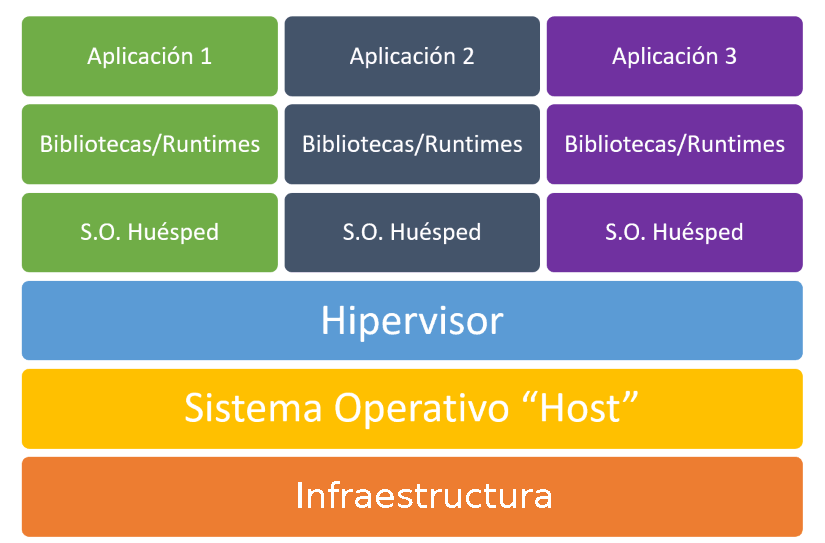
\includegraphics[width=0.4\textwidth]{imagenes/entorno/virtual.png}
	\caption{Arquitectura de un entorno virtual} \label{virtual}
\end{figure}
Por debajo del sistema operativo siempre estará la infraestructura, por ejemplo el ordenador personal para realizar cualquier desarrollo, o si es por ejemplo un despliegue real se usará un servidor.

Para que una \textbf{máquina virtual} pueda ejecutarse es necesario la instalación del \textbf{hipervisor} que se trata de un software especializado en exponer los recursos hardware que están debajo del sistema operativo, de forma que puedan ser utilizados por otros sistemas operativos. Los hipervisores vienen como productos como Hyper-V, VirtualBox o VMWare, entre otros.

Gracias a todo esto podemos tener diferentes sistemas operativos ejecutándose en paralelo sobre la misma máquina física, cada uno con su memoria y espacio en disco reservados, y completamente aislados unos de otros.
\subsubsection{Aplicación de contenedores}

La filosofía de los contenedores es totalmente diferente a la de las máquinas virtuales. Si bien tratan también de aislar a las aplicaciones y de generar un entorno replicable y estable para que funcionen, en lugar de albergar un sistema operativo completo lo que hacen es compartir los recursos del propio sistema operativo "host" sobre el que se ejecutan.
\newpage
Su esquema viene estructurado de la forma en la que viene representado en la figura \ref{contenedores}.

\begin{figure}[H]
	\centering
	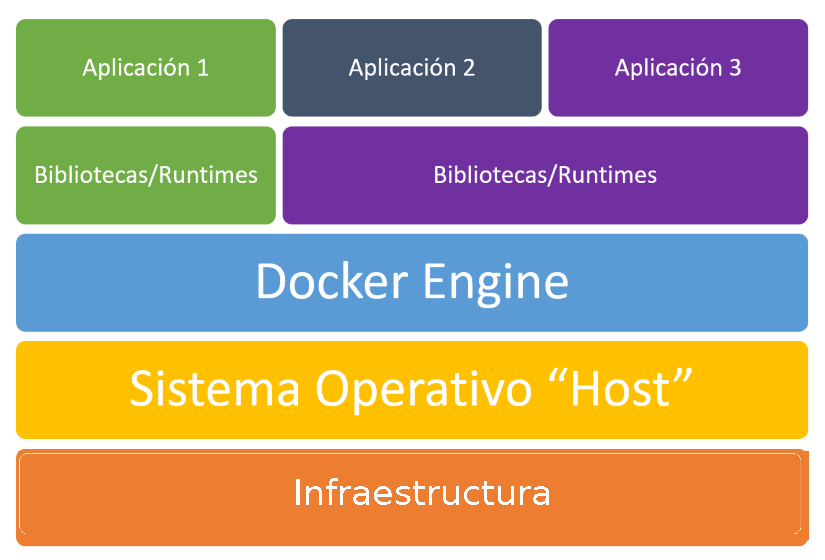
\includegraphics[width=0.4\textwidth]{imagenes/entorno/contenedores.png}
	\caption{Estructura de un entorno con contenedores} \label{contenedores}
\end{figure}
En primer lugar debemos tener en cuenta que, en el caso de los contenedores, el hecho de que no necesiten un sistema operativo completo sino que reutilicen el subyacente reduce mucho la carga que debe soportar la máquina física, el espacio de almacenamiento utilizado y el tiempo necesario para lanzar las aplicaciones. Por lo tanto los contenedores son mucho más ligeros que las máquinas virtuales.

Cuando definimos una máquina virtual debemos indicar de antemano cuántos recursos físicos le debemos dedicar. En el caso de los contenedores esto no es así. De hecho no indicamos qué recursos vamos a necesitar, sino que en función de las necesidades de cada momento, el encargado de asignar lo que sea necesario para que los contenedores funcionen adecuadamente.

Esto hace que los entornos de ejecución en contenedores sean mucho más ligeros, y que se aproveche mucho mejor el hardware, además de permitir levantar muchos más contenedores que máquinas virtuales en la misma máquina física. Mientras que una máquina virtual puede tardar un minuto o más en arrancar y tener disponible nuestra aplicación, un contenedor se levanta y responde en unos pocos segundos. El espacio ocupado en disco es muy inferior con los contenedores al no necesitar que instalemos el sistema operativo completo.

Además para realizar despliegues avanzados de aplicaciones en contenedores hay que ir más allá y utilizar tecnologías que nos permiten orquestar y controlar los despliegues con muchas partes en ejecución.

Como desventajas se tiene que no pueden sustituir por completo la virtualización tradicional y no todo el mundo cuenta de un modelo de negocio que sea compatible a estos.

También aumentan riesgos de brechas de seguridad, además cuentan con menos flexibilidad a nivel de sistema operativo del contenedor.

Dejar de usar sistemas operativos separados implica una mejora en el rendimiento de la virtualización con contenedores, pero significa también tener un nivel más bajo de seguridad. En una virtualización del sistema operativo tienen efecto sobre todos los contenedores. 

Todas las soluciones de \textbf{virtualización de contenedores Linux} actuales basan su funcionamiento en una serie de librerias o funcionalidades básicas del kernel y vertebran la arquitectura que da soporte a su funcionamiento. Estos componentes son:

\begin{itemize}
	\item  \textbf{CGROUPs}: se trata de una característica del kernel que permite limitar los recursos del sistema, es decir, limita, contabiliza y aisla el uso de los recursos como puede ser la CPU, la memoria, el disco, etc, para un conjunto de procesos.
	\item \textbf{NAMESPACES}: es un espacio donde uno o mas identificadores de proceso pueden co-existir. Esto permite que tengamos varios PID’s agrupados, pero separados de otros sin que puedan ver qué recursos están utilizando cada uno de los espacios de nombres adyacentes. Existen 6 tipos básicos de \textbf{namespaces} relacionados con
	distintos aspectos del sistema:
	\begin{itemize}
		\item \textbf{NETWORK namespace}: Aislamiento de red. Así, cada namespace de red tendrá sus propias interfaces, direcciones y puertos de red, tablas de enrutamiento,
		etc.
		\item \textbf{PID namespace}: Aísla el espacio de identificadores de proceso. Un contenedor
		tendrá su propia jerarquía de procesos y su proceso padre o init (PID 1).
		\item \textbf{UTS namespace}: Aísla el dominio y hostname, permitiendo a un contenedor
		poseer su propio dominio de nombres.
		\item \textbf{MOUNT namespace}: Aísla los puntos de montaje de los sistemas de ficheros
		que puede ver un grupo de procesos. Este namespace fue el punto de partida,con chroot.
		\item \textbf{USER namespace}: Aísla identificadores de usuarios y grupos. Así dentro un
		contenedor es posible tener un usuario con ID 0 (root) que se corresponda con
		un ID de usuario cualquiera en el host.
		\item \textbf{IPC namespace}: Aísla la intercomunicación entre procesos dentro del espacio
	\end{itemize}
\end{itemize}

En este trabajo usaremos los contenedores por las ventajas mencionadas. A continuación explicaremos algunas herramientas que permiten automatizar aplicaciones a través de contenedores: 
\paragraph{Docker Engine}
\textbf{Docker} \cite{docker} \cite{dockerCE} se trata de un proyecto de software libre que permite automatizar el despliegue de aplicaciones dentro de contenedores. Permitiendo empaquetar una aplicación en una unidad estandarizada para el desarrollo de software, que contiene todo lo necesario para su funcionamiento.
\begin{figure}[H]
	\centering
	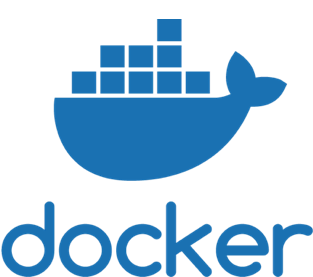
\includegraphics[width=0.4\textwidth]{imagenes/entorno/docker.png}
	\caption{Docker} \label{docker}
\end{figure}

Usa recursos del sistema de forma totalmente aislada, permitiendo asignar recursos o combinaciones de estos recursos entre los procesos que se ejecutan en un sistema.

Los contenedores de imagen de \textbf{Docker} se pueden ejecutar de forma nativa en Linux y Windows. Sin embargo, las imágenes de Windows solo pueden ejecutarse en hosts de Windows y las imágenes de Linux pueden ejecutarse en hosts de Linux y hosts de Windows, donde host significa un servidor o una máquina virtual.

Permite centrarse en el código sin preocuparse de si funcionará en la máquina en la que se ejecutará. Esto acelera el proceso de mantenimiento y desarrollo de cada proyecto y, de cara a DevOps, permite que tanto los desarrolladores como los administradores de sistema pueden probar aplicaciones en un entorno seguro y exactamente igual en todos los casos.

A nivel de arquitectura y componentes, \textbf{Docker} funciona de forma que para proporcionar las características básicas de aislamiento y virtualización emplea las tecnologías que proporciona el Kernel de Linux.

Es un sistema que permite una enorme \textbf{portabilidad} ya que, debido al enorme auge que ha experimentado, la mayor parte de las grandes empresas comerciales de tecnologías de infraestructuras orientadas al cloud computing permiten ejecutar contenedores Docker de forma nativa desde sus plataformas cloud. Destacamos el caso de \textbf{Google Cloud, Amazon AWS y Microsoft Azure} que tienen plataformas nativas especializadas en la ejecución de contenedores Docker con múltiples funcionalidades y tipos de escalabilidad y alta disponibilidad.

Auspiciado por el éxito de las soluciones \textbf{Docker}, podemos encontrar en el mercado un gran numero de aplicaciones comerciales en formato contenedor Docker para ser usadas y arrancadas sin necesidad de conocimientos previos. Del mismo modo, podemos encontrar todo tipo de servicios que se distribuyen preparados para ser usados en formato contenedor Docker, lo que nos permite acceder a desplegar una enorme cantidad de aplicaciones y servicios sin
prácticamente necesidad de un conocimiento previo de los pasos de su instalación, y lo que es más importante, con el soporte directo del fabricante de la solución.

Podemos ver a \textbf{Docker} además de como una herramienta para la creación de contenedores virtuales, como una capa más de abstracción y aislamiento que además aporta un sistema que facilita enormemente la gestión y administración de los contenedores.
\paragraph{OpenShift}
Software creado por \textbf{Red Hat}, fabricante detrás de una de las distribuciones Linux comerciales más extendidas, OpenShift es una solución que permite desplegar aplicaciones realizadas con cualquier stack de tecnologías.\cite{openshift}
\begin{figure}[H]
	\centering
	
\includegraphics[width=0.4\textwidth]{imagenes/entorno/openshift.png}
	\caption{OpenShift} \label{openshift}
\end{figure}
Básicamente, permite al desarrollador centrarse en su trabajo de creación de la aplicación y evitar preocuparse con el mantenimiento de los servicios o la escalabilidad de las aplicaciones. Es capaz de trabajar con lenguajes y frameworks diversos y permite modificar y desplegar las aplicaciones rápidamente bajo demanda, automatizando el proceso entero.

Cuenta con una interfaz bastante intuitiva y manejable. \textbf{Openshift} se basa en Docker y Kubernetes, pero añade una nueva capa.

Es ahora mismo una de las opciones más interesantes para \textbf{Cloud privadas}, ya que está basada en estándares abiertos, integra con las tecnologías open source de referencia y tiene un market en constante crecimiento. 

Aunque está basada en código abierto, y cuenta con versiones gratuitas, no deja de ser un producto de \textbf{RedHat}. Por lo que contará con versiones de pago. 

Como desventaja es que no deja instalar ciertas imágenes o utilizar el usuario root. Cuenta con gestión de imágenes de contenedores con \textbf{ImageStreams} Además tiene integración de la herramienta \textbf{Jenkins}.

\paragraph{CoreOS rkt (rocket)}
Es un  motor de software de automatización de contenedores para ejecutar cargas de trabajo de aplicaciones de forma aislada de la infraestructura subyacente.\cite{rkt}

\begin{figure}[H]
	\centering
	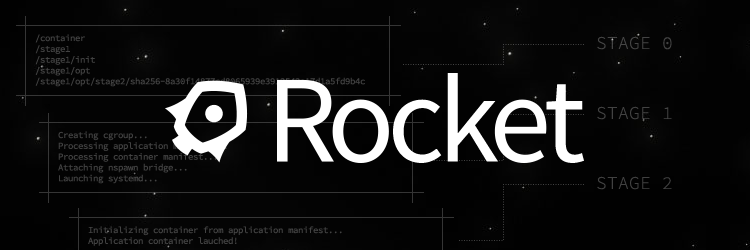
\includegraphics[width=0.4\textwidth]{imagenes/entorno/rocket.png}
	\caption{CoreOS} \label{rocket}
\end{figure}

Los contenedores CoreOS rkt operan en la mayoría de las principales distribuciones del sistema operativo Linux como un archivo binario que se integra con los sistemas y scripts de inicio de Linux, y opera de acuerdo con el modelo de proceso estándar de Unix, que es una relación padre-hijo. 

Respecto a CoreOS Rkt, este sistema es similar a Docker ya que se encarga de la virtualización de aplicaciones en el propio sistema operativo principal.
\newpage
Algunas de las principales características de este software es que también se ha diseñado pensando en la seguridad por defecto, incluye soporte para \textbf{SELinux} así como para ejecutar aplicaciones en máquinas virtuales aisladas. Otras características es que soporta varios sistemas de inicio como systemd y upstart, por último, también puede ejecutar imágenes Docker.

Como inconvenientes es que existen muchas menos integraciones de proveedores externos para \textbf{rkt} que para Docker.

Además \textbf{rkt} está optimizado para operar contenedores de aplicaciones, pero no soporta contenedores de sistemas operativos (full system container).
\paragraph{LXC (Linux Containers)}
A diferencia de Docker y CoreOs rkt, \textbf{LXC} es una tecnología de sistema que se encarga de generar contenedores de sistema.\cite{lxc} 

\begin{figure}[H]
	\centering

\includegraphics[width=0.4\textwidth]{imagenes/entorno/lxc.png}
	\caption{LXC} \label{lxc}
\end{figure}

El que compartan el kernel otorga menos aislamiento al sistema principal y además le da acceso a los recursos de la máquina anfitriona, pero queda parcialmente limitado por espacios de procesos y de red.

Como \textbf{desventaja} podemos decir que no se utiliza de forma estándar para operar contenedores de aplicaciones. A excepción de Linux, no cuenta con ninguna implementación nativa para otros sistemas operativos. Esto es que también podemos ejecutarlo en otros sistemas operativos, como puede ser Mac o Windows, pero siempre como resultado de ejecutarlos embebidos dentro de un entorno Linux que se virtualiza de forma clásica sobre un anfitrión con otro sistema operativo. 
\newpage
Por este motivo, se considera que no es una ejecución nativa ya que es necesario virtualizar primero el sistema operativo Linux para poder, dentro de este, virtualizar contenedores.
\subsection{Alternativa elegida: Uso de contenedores con Docker}
Después de exponer todas las alternativas anteriores usaremos \textbf{Docker} por las siguientes razones:
\begin{itemize}
	\item En cuanto al peso, es el más ligero ya que automatiza aplicaciones con muy poco espacio.
	\item Se puede desplegar cualquier contenedor en cualquier otro sistema, con lo que se ahorra el tener que instalar de nuevo los entornos.
	\item Es más seguro ya que utiliza por defecto la máxima confianza probable para que el software que contiene se ejecute en un ambiente totalmente controlado.
	\item Usa libcontainer que es un derivado de LXC, que se trata de una abstracción para admitir una gama más amplia de tecnologías de aislamiento.
	\item Permite una consola interactiva para el usuario.
	\item Es la opción más recomendada para montar entornos ad-hoc con tecnologías open source, ya sea en nubes públicas o privadas.
	
\end{itemize}
\section{Desarrollo del despliegue de Naemon}
En cuanto al software utilizado, el equipo cuenta con un sistema operativo \textbf{Pop!\_OS 18.04} y al que se le ha realizado la instalación de \textbf{Docker}. 

\textbf{Pop!\_OS} se basa en Ubuntu, de la que toma sus dos grandes fundamentos: Linux 5.0 y GNOME 3.32. Cuenta con mejor soporte de hardware, mejor rendimiento y más opciones de configuración.
\newpage
Por otro lado, el escritorio escapa de la disposición del de Ubuntu y se acerca al estilo de GNOME, complementándolo con su propio tema de aplicaciones e iconos, algunos de los cuales han sido rediseñados para esta versión siguiendo las líneas de diseño de GNOME, con diversas extensiones preinstaladas, para poder tener los iconos en el escritorio o para gestionar la batería.

\textbf{Pop!\_OS} ofrece la posibilidad de reinstalar el sistema sin perder usuarios o datos. La distribución sigue las versiones de Ubuntu, pero no está enfocada en la reinstalación, sino en la actualización constante de una versión a otra con excepción de la LTS, para la que siguen manteniendo algunos de sus paquetes.

Además cuenta con dos formas de instalación o adaptación uno para \textbf{Intel/AMD} y otro para \textbf{Nvidia}.

El contenedor creado lanzará Naemon sobre una base Ubuntu Bionic (18.04).

La imagen base que utilizaremos será una versión minimalista de Ubuntu Bionic obtenida desde:\\
 \url{https://github.com/phusion/baseimage-docker}.

Tienes Ubuntu instalado en Docker. Los archivos están ahí. Pero eso no significa que Ubuntu esté funcionando como debería.

Cuando se inicia su contenedor Docker, solo se ejecuta el comando CMD. Los únicos procesos que se ejecutarán dentro del contenedor es el comando CMD y todos los procesos que genera. Es por eso que todo tipo de servicios importantes del sistema no se ejecutan automáticamente: debe ejecutarlos usted mismo.

Su sistema de inicio, \textbf{Upstart}, asume que se está ejecutando en hardware real o virtualizado, pero no dentro de un contenedor Docker. Por eso utilizaremos esta imagen de \textbf{phusion}.

Esta imagen incluye la forma de iniciar el proceso de inicio de forma correcta, esto es que viene con un proceso de inicio \textbf{/sbin/my\_init} que cosecha los procesos secundarios huérfanos correctamente y responde a \textbf{SIGTERM} correctamente. De esta manera, el contenedor no se llenará de procesos \textbf{zombies} y el comando \textbf{docker stop}funcionará correctamente.
\newpage
Además soluciona \textbf{incompatibilidades APT con Docker}. Se encarga de ejecutar un demonio \textbf{syslog} para que los mensajes importantes del sistema no se pierdan.Otra tarea que incluye es que ejecuta un demonio cron para que los cronjobs funcionen.Cuenta con un \textbf{servidor SSH} que le permite iniciar sesión fácilmente en su contenedor para inspeccionar o administrar cosas. El \textbf{daemon SSH} está deshabilitado de forma predeterminada.

Cuenta con el demonio runit que es utilizado para la supervisión y gestión de servicios. Mucho más fácil de usar que \textbf{SysV init} \cite{SysVinit} y admite reiniciar demonios cuando se bloquean. Mucho más fácil de usar y más liviano que \textbf{Upstart}.

Incluye una herramienta personalizada para ejecutar un comando como otro usuario. Es más fácil de usar que su, tiene un vector de ataque más pequeño que sudo, y a diferencia de \textbf{chpst} esta herramienta configura \textbf{\$HOME} de forma correcta. Disponible como \textbf{/sbin/setuser}.
\begin{figure}[H]
	\centering
	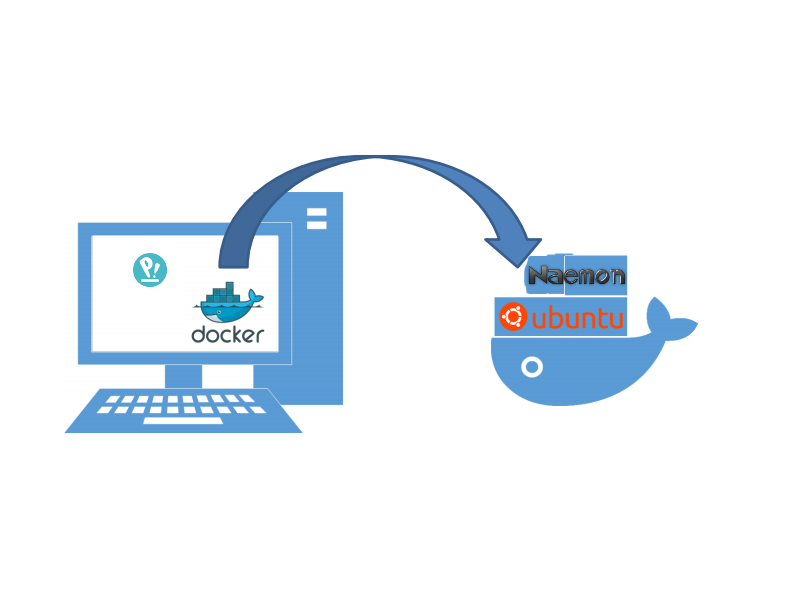
\includegraphics[width=0.9\textwidth]{imagenes/despliegue_naemon/docker_naemon.png}
	\caption{Estructura del contendor Docker con Naemon y Ubuntu de forma minimalista} \label{dockernaemon}
\end{figure}
\newpage
\section{Creación de Dockerfile}

Para poder realizar el despliegue tendremos que crear el fichero \textbf{Dockerfile}. Con este fichero construiremos la imagen de Naemon de forma automática, leyendo las instrucciones que le indiquemos.

Se trata de un documento de texto que contiene todas las órdenes a las que un usuario dado puede llamar, desde la línea de comandos, para crear una imagen.

Los pasos principales para crear una imagen a partir de un fichero Dockerfile son:

\begin{itemize}
	\item Crear un nuevo directorio que contenga el fichero, con el guión y otros ficheros que fuesen necesarios para crear la imagen.
	\item Crear el contenido.
	\item Construir la imagen mediante el comando docker build.
\end{itemize}

La sintaxis para el comando es:

\begin{lstlisting}[language=bash]
$ docker build [opciones] RUTA | URL | -
\end{lstlisting}


Las opciones más comunes son:
\begin{itemize}
	\item \textbf{-t}, nombre [:etiqueta]. Crea una imagen con el nombre y la etiqueta especificada a partir de las instrucciones indicadas en el fichero. Se recomienda usar este parámetro cuando se quiere asingar un nombre a la imagen.
	\item \textbf{–no-cache}. Por defecto, Docker guarda en memoria caché las acciones realizadas recientemente. Si se diese el caso de que ejecutamos un docker build varias veces, Docker comprobará si el fichero contiene las mismas instrucciones y, en caso afirmativo, no generará una nueva imagen. Para generar una nueva imagen omitiendo la memoria caché utilizaremos siempre esta opción.
	\item \textbf{–pull}. También por defecto. Docker solo descargará la imagen especificada en la expresión FROM si no existe. Para forzar que descargue la nueva versión de la imagen utilizaremos esta opción.
	\item \textbf{–quiet}. Por defecto, se muestra todo el proceso de creación, los comandos ejecutados y su salida. Utilizando esta opción solo mostrará el identificador de la imagen creada.
\end{itemize}

\begin{figure}[H]
	\centering
	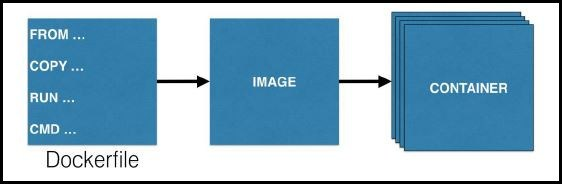
\includegraphics[width=0.9\textwidth]{imagenes/despliegue_naemon/dockerfile-image.png}
	\caption{Estructura de un fichero Dockerfile} \label{dockerfile}
\end{figure}
Para crear este fichero \textbf{Dockerfile} como el figurado en \ref{dockerfile} antes tenemos que aprender los comandos disponibles:
\begin{itemize}
	\item \textbf{MAINTAINER} : Nos permite configurar datos del autor, principalmente su nombre y su dirección de correo electrónico.
	\item \textbf{ENV} : Configura las variables de entorno.
	\item  \textbf{ADD} : Esta instrucción se encarga de copiar los ficheros y directorios desde una ubicación especificada y los agrega al sistema de ficheros del contenedor. Si se trata de añadir un fichero comprimido, al ejecutarse el guión lo descomprimirá de manera automática.
	\item  \textbf{COPY} : Es la expresión recomendada para copiar ficheros, similar a ADD.
	\item  \textbf{EXPOSE} : Indica los puertos en los que va a escuchar el contenedor. Hay que tener en cuenta que esta opción no consigue que los puertos sean accesibles desde el host; para esto debemos utilizar la exposición de puertos mediante la opción -p de docker run, tal y como explicamos en un artículo anterior.
	\item  \textbf{VOLUME} : Esta es una opción que muchos usuarios de la Web estaban esperando como agua de mayo. Nos permite utilizar en el contenedor una ubicación de nuestro host, y así, poder almacenar datos de manera permanente. Los volúmenes de los contenedores siempre son accesibles en el host anfitrión, en la ubicación: \textbf{/var/lib/docker/volumes/}
	\item  \textbf{WORKDIR} : El directorio por defecto donde ejecutaremos las acciones.
	\item  \textbf{USER} : Por defecto, todas las acciones son realizadas por el usuario root. Aquí podemos indicar un usuario diferente.
	\item  \textbf{SHELL} : En los contenedores, el punto de entrada es el comando \textbf{/bins/sh -c} para ejecutar los comandos específicos en CMD, o los comandos especificados en línea de comandos para la acción run.
	\item  \textbf{ARG} : Podemos añadir parámetros a nuestro Dockerfile para distintos propósitos.
\end{itemize}
A continuación indicaremos los pasos a seguir para instalar Naemon y la forma en que se ha indicado en dicho \textbf{Dockerfile}.
\subsection{Instalación de imagen base phusion}
La base de descarga será la siguiente \url{https://github.com/phusion/baseimage-docker}, donde podemos encontrar que dicha base es más eficiente que las bases comunes de Docker conocidas como \textbf{Alpine} y \textbf{BusyBox} en cuanto a la entrada y salida de sus datos de red. 
\begin{figure}[H]
	\centering
	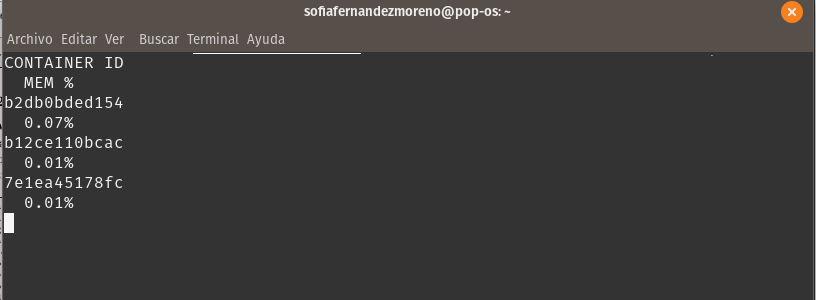
\includegraphics[width=0.9\textwidth]{imagenes/despliegue_naemon/estadisticasRAM.png}
	\caption{Comparativas de estadísticas} \label{phusion}
\end{figure}
En la figura \ref{phusion} se referencia al nombre \textbf{hungry\_poitras} con la imagen de la base de \textbf{phusion}, el nombre de \textbf{vigorous\_wing} con \textbf{Busybox} y \textbf{objective\_crazy} con \textbf{Alpine}.
\newpage
Por lo que tendremos que añadir en el Dockerfile las siguientes líneas:
\begin{lstlisting}[language=bash]
FROM phusion/baseimage:0.11
MAINTAINER Sofia <chui274@gmail.com>
\end{lstlisting}
\subsection{Instalación paquetes}
Debemos instalar las dependencias y los paquetes para que Naemon se pueda ejecutar perfectamente. Para ello debemos instalar el entorno LAMP en donde vayamos a aplicar Naemon. El comando que introduciremos en nuestro Dockerfile será el siguiente:
\begin{lstlisting}[language=bash]
RUN apt-get update && \
DEBIAN_FRONTEND=noninteractive \
apt-get install -y \
apache2\
apache2-utils\
libapache2-mod-fcgid\
libfontconfig1\
libjpeg62\
libgd3\
libxpm4\
xvfb\
ssmtp\
ruby\
python2.7\
python-boto\
perl\
libwww-perl\
libcrypt-ssleay-perl
\end{lstlisting}

Al principio le hemos indicado actualizar los repositorios por si existe alguna versión reciente en nuestro sistema.

Además hemos indicado para usar la sentencia siguiente:
\begin{lstlisting}[language=bash]
DEBIAN_FRONTEND=noninteractive
\end{lstlisting}
para indicar que queremos instalar y establecer el entorno apt-get de forma no interactivo y usar el script de shell en Dockerfile.
\newpage
\subsection{Instalación clave GPG}
El siguiente paso a seguir es agregar el repositorio de \textbf{Consol Labs} para crear la base de datos apt. Para ello debemos importar la clave GPG y así seguidamente generaremos las claves públicas para los servidores.

Por lo que habrá que añadir al documento \textbf{Dockerfile} las siguientes líneas para realizar lo anterior especificado:

\begin{lstlisting}[language=bash]
RUN   curl -s "https://labs.consol.de/repo/stable/RPM-GPG-KEY" | apt-key add -
RUN   gpg --keyserver keys.gnupg.net --recv-keys F8C1CA08A57B9ED7
RUN   gpg --armor --export F8C1CA08A57B9ED7 | apt-key add -
RUN   echo "deb http://labs.consol.de/repo/stable/ubuntu $(lsb_release -cs) main" > /etc/apt/sources.list.d/labs-consol-stable.list

\end{lstlisting}
\subsection{Instalación repositorio}
Realizado la instalación de la clave GPG debemos actualizar los repositorios y una vez actualizados los repositorios instalaremos la aplicación Naemon, además de que instalaremos los plugins correspondientes de Nagios que son compatibles con este, para ello introduciremos los siguientes comandos al Dockerfile:


\begin{lstlisting}[language=bash]

RUN apt-get update &&\
DEBIAN_FRONTEND=noninteractive apt-get install -y \
nagios-nrpe-plugin\
naemon=1.0.10


\end{lstlisting}

Le volvemos a indicar que queremos el entorno de forma no interactiva, además a la hora de realizar las instalaciones se le indicará, a través del \textbf{parámetro -y}, que confirmamos la instalación, ya que si no se confirma con anterioridad no realizará la creación de la imagen ya que no Docker no ofrece los permisos suficientes.

\subsection{Inicialización de directorios}
Una vez finalizada la instalación de Naemon, tendremos que indicar los directorios en los que vamos a trabajar, ya que el usuario desconoce los directorios internos de Naemon, para ello realizaremos la inicialización del directorio de datos creando unas variables de entorno. 
\newpage
Para ello crearemos un archivo llamado \textbf{data\_dirs.env} donde se recorrerá la variable global \textbf{DATA\_DIRS} que se compondrá de los directorios que queremos tener en nuestro contenedor, es decir, para poder tener acceso a los directorios con los que vamos a trabajar.

Dicho archivo .env permite personalizar las variables de entorno de trabajo individuales. Como hemos mencionado recorreremos la variable  \textbf{DATA\_DIRS} ingresando los directorios:

\begin{itemize}
	\item /etc/naemon
	\item /var/log/naemon
	\item /etc/thruk
	\item /var/log/thruk
	\item /usr/lib/naemon/plugins
\end{itemize}

Introduciremos dentro de la variable para agregar también el directorio de instalación de Thruk.

La forma de ir introduciendo los directorios lo haremos a través de forma de lenguaje bash de la siguiente manera:

\begin{lstlisting}[language=bash]
i=0
DATA_DIRS[((i++))]="/etc/naemon"
DATA_DIRS[((i++))]="/var/log/naemon"
DATA_DIRS[((i++))]="/etc/thruk"
DATA_DIRS[((i++))]="/var/log/thruk"
DATA_DIRS[((i++))]="/var/www"
DATA_DIRS[((i++))]="/usr/lib/naemon/plugins"
export DATA_DIRS


\end{lstlisting}

\subsubsection{Creación script de inicialización: init.bash}
Ahora una vez creada la variable de entorno con la que vamos a trabajar para poder operar con los directorios necesitamos inicializar el diseño del directorio de datos personalizado, para ello crearemos un script bash donde nos encargaremos de incluir en una variable \textbf{\textit{datadir}} todos los datos recogidos de la variable de entorno y moverlos a la plantilla de cada directorio, seguidamente realizaremos un enlace simbólico entre los directorios creados y los directorios reales.
\newpage
Es decir, a través del fichero \textbf{data\_dirs.env} accederemos a la variable de entorno \textbf{DATA\_DIRS} y por cada iteración del mismo moveremos dichas rutas a una plantilla y luego como hemos mencionado se creará el enlace simbólico.

El script es el siguiente:

\begin{lstlisting}[language=bash]
#!/bin/bash

source /data_dirs.env

mkdir -p /data
for datadir in "${DATA_DIRS[@]}"; do
mv ${datadir} ${datadir}-template
ln -s /data/${datadir#/*} ${datadir}
done

\end{lstlisting}
\subsubsection{Copia de archivos}
A través de Dockerfile y con el comando ADD copiaremos los archivos anteriores data\_dirs.env e init.bash a sus repestivos, es decir, realizaremos lo siguiente:
\begin{lstlisting}[language=bash]
ADD data_dirs.env /data_dirs.env
ADD init.bash /init.bash
\end{lstlisting}
Con esto queremos copiar el contenido de data\_dirs.env en el nuevo archivo /data\_dirs.env, al igual pasa con init.bash que copiaremos su contenido en la raíz del contenedor, es decir, en /init.bash.

Esto lo realizaremos para que el \textbf{Dockerfile pueda tener acceso a dichos datos y así poder operar}, ya que por defecto Docker no sabe de la existencia de dichos archivos sino los introducimos en el contenedor.

\subsubsection{Asignación de permisos}
Para poder ejecutar dicho script init.bash es necesario asignar una serie de permisos, para ello le indicaremos que queremos asignarle el permiso 755, es decir, este permiso se ocupa de que el propietario del fichero pueda leer, escribir y ejecutar el archivo. Todos los otros puedan leer y ejecutar el archivo. Este ajuste es común para los programas que son utilizados por todos los usuarios.
\newpage
Además le indicaremos también a través del comando sync que fuerce la grabación de los datos de la caché y así solventar la presencia de errores y reducir el tamaño de procesamiento.
Esto lo indicaremos en el fichero Dockerfile de la siguiente forma:
\begin{lstlisting}[language=bash]
RUN chmod 755 /init.bash &&\
sync && /init.bash &&\
sync && rm /init.bash
\end{lstlisting}

Además le indicaremos que ejecute el script init.bash para poder inicializar la información de los directorios.

\subsection{Cargar datos en carpeta raíz}
Como se mencionó anteriormente se creaba el directorio \textbf{data}, entonces para poder trabajar con el contenedor estableceremos el punto de montaje de Naemon en dicho directorio eso lo realizaremos con el comando \textbf{VOLUME} de Docker, que básicamente creará un punto de montaje con el nombre especificado y lo marca como que contiene volúmenes montados externamente desde el host nativo u otros contenedores.

 El valor puede ser una \textbf{\textit{matriz JSON}}, por ejemplo,\textbf{ VOLUME [``/var/log/"]} o una cadena simple con varios argumentos, como \textbf{VOLUME /var/logo}.
Cuando realicemos el comando \textbf{\textit{run}} de Docker, se inicializará el volumen recién creado con cualquier dato que exista en la ubicación especificada dentro de la imagen base.
Por lo tanto esto lo realizaremos en el fichero Dockerfile de la siguiente manera:
\begin{lstlisting}[language=bash]
VOLUME ["/data"]
\end{lstlisting}
\subsection{Protocolo de salida}
Para poder utilizar Naemon en un servidor web debemos realizar una conexión a través de los nodos y para ello utilizaremos el protocolo \textbf{TCP} desde el puerto 80 de HTTP.

Esto se podrá realizar a través de EXPOSE, qu su función es la de informar a Docker que el contenedor escucha en los puertos de red especificados en el tiempo de ejecución. Puede especificar si el puerto escucha en TCP o UDP, y el valor predeterminado es TCP si no se especifica el protocolo.
\newpage
Dicha instrucción no publica realmente el puerto. Funciona como un tipo de documentación entre la persona que construye la imagen y la persona que ejecuta el contenedor, acerca de los puertos que deben publicarse.

Para publicar realmente el puerto cuando se ejecuta el contenedor, se debe usar el flag \textbf{-p} en el comando docker run para publicar y asignar uno o más puertos, o el flag \textbf{-P} para publicar todos los puertos expuestos y asignarlos a puertos de alto orden.

Por defecto, EXPOSE asume TCP. También puede especificar UDP. En nuestro Dockerfile usaremos la siguiente línea para comunicar con TCP.

\begin{lstlisting}[language=bash]
EXPOSE 80/tcp
\end{lstlisting}
\subsection{Creación de imagen y ejecución de Dockerfile}
En esta sección especificaremos como podemos ejecutar a través de los propios comandos de Docker nuestra imagen, para ello realizaremos los siguientes pasos:
\subsubsection{Creación de ENTRYPOINT}
Primero utilizaremos el comando ENTRYPOINT en nuestro Dockerfile, ya que la funcionalidad de este es permitir configurar un contenedor que se ejecutará como un tipo de ejecutable. ENTRYPOINT puede tener dos formas:
\begin{itemize}
	\item \textbf{ENTRYPOINT [ejecutable,parametro]} Formato ejecutable
	\item \textbf{ENTRYPOINT comando parametro} Formato shell
\end{itemize}	
En nuestro caso se ha elegido la primera opción, ya que previamente hemos creado un fichero bash donde realizaremos las ejecuciones que contaremos a continuación. Previamente se ha creado en el Dockerfile las líneas para copiar dicho bash en la raíz del contenedor y darle la asignación de permisos de tipo 755 a dicho bash:
\begin{lstlisting}[language=bash]
ADD run.bash /run.bash
RUN chmod 755 /run.bash
\end{lstlisting}
\newpage
\paragraph{Fichero bash de ejecución: run.bash}

Anteriormente ejecutábamos la asignación de permisos de ejecución del fichero run.bash, para realizar la ejecución realizamos:
\begin{lstlisting}[language=bash]
ENTRYPOINT ["/run.bash"]
\end{lstlisting}

Con esto ejecutará dicho fichero bash que vamos a comentar a continuación:

Primero realizaremos la configuración de Naemon de forma externa a través del volumen \textbf{/data}
\begin{lstlisting}[language=bash]

source /data_dirs.env
DATA_PATH=/data

for datadir in "${DATA_DIRS[@]}"; do
	if [ ! -e "${DATA_PATH}/${datadir#/*}" ]
	then
		echo "Installing ${datadir}"
		mkdir -p ${DATA_PATH}/${datadir#/*}
		if [ "$(ls -A ${datadir}-template 2> /dev/null)"  ]
		then
			cp -pr ${datadir}-template/* ${DATA_PATH}/${datadir#/*}/
		fi
	fi
done

\end{lstlisting}

Para ello recorremos cada una de las instancias del volumen e iremos creando los directorios, solo si no existe el directorio. Seguido comprobamos que no exista un enlace simbólico, si de verdad no existe, copiaremos el contenido del directorio template dentro del directorio datadir.

En versiones antiguas de Naemon la contraseña del archivo htpasswd de thruk se guardaba en el archivo /etc/naemon, a través de nuestro script run comprobaremos que si es una versión antigua y se encuentra en dicha carpeta lo traslade al archivo /etc/thruk/htpasswd.

\begin{lstlisting}[language=bash]
if [ -e /etc/naemon/htpasswd ]
then
echo "UPGRADE: Moving the htpasswd file to the new location..."
mv /etc/naemon/htpasswd /etc/thruk/htpasswd
# We assume the naemon password was set in an upgrade situation
touch /etc/thruk/._install_script_password_set
fi
\end{lstlisting}

Por defecto se asigna el usuario y contraseña \textbf{thrukadmin} dentro del fichero /etc/thruk/htpasswd.
\newpage
Si no queremos que esa sea la contraseña asignada, podemos crear dentro del script una combinación para crear una contraseña aleatoria, para ello usaremos la variable RANDOM\_PASS y WEB\_ADMIN\_PASSWORD donde se asignará dicha contraseña.

A través de la siguientes líneas realizaremos lo comentado:


\begin{lstlisting}[language=bash]
RANDOM_PASS=`date +%s | md5sum | base64 | head -c 8`
WEB_ADMIN_PASSWORD=${WEB_ADMIN_PASSWORD:-$RANDOM_PASS}
htpasswd -bc /etc/thruk/htpasswd thrukadmin ${WEB_ADMIN_PASSWORD}
echo "Set the thrukadmin password to: $WEB_ADMIN_PASSWORD"
touch /etc/thruk/._install_script_password_set
\end{lstlisting}


Ahora nos encargaremos de comprobar que si estamos actualizando desde un contenedor anterior, moveremos el archivo llamado \textbf{cgi.cfg} a una nueva localización. Es decir, moveremos desde la ruta /etc/naemon/cgi.cfg a /etc/thruk/cgi.cfg.

A continuación se creará una función para realizar la parada del servidor apache y matar el proceso Naemon.

Realizamos por tanto lo siguiente:

\begin{lstlisting}[language=bash]
function salida_exitosa(){
/etc/init.d/apache2 stop
pkill naemon
exit $1
}
\end{lstlisting}

Hay que señalar que la imagen de phusion no funciona el comando \textbf{service naemon stop} por lo que habrá que realizar lo anterior.

Ahora nos aseguramos de dar los permisos de propiedad al volumen creado, es decir, a \textbf{data}, incluso si se cambian los UID o GID.

\begin{lstlisting}[language=bash]
chown -R naemon:naemon /data/etc/naemon /data/var/log/naemon
chown -R www-data:www-data /data/var/log/thruk /data/etc/thruk
\end{lstlisting}


Asignamos el permiso 775 al directorio /var/cache/naemon ya que no es editable por otros usuarios que no sean naemon, lo que significa que la herramienta de configuración de thruk no puede escribir en el directorio para verificaciones de configuración.

\begin{lstlisting}[language=bash]
chmod 775 /var/cache/naemon
\end{lstlisting}
\newpage
Solo nos quedará iniciar los servicios de Naemon y Apache con:

\begin{lstlisting}[language=bash]
service naemon start
service apache2 start
\end{lstlisting}

Anteriormente habíamos realizado una función para realizar una salida exitosa, ahora haremos uso de dicha función comprobando si naemon o apache está funcionando o no:
\begin{lstlisting}[language=bash]
trap "salida_exitosa 0;" SIGINT SIGTERM

while true
do
service naemon status > /dev/null
if (( $? != 0 ))
then
echo "Naemon no longer running"
salida_exitosa 1
fi

/etc/init.d/apache2 status > /dev/null
if (( $? != 0 ))
then
echo "Apache no longer running"
salida_exitosa 2
fi
sleep 1
done
\end{lstlisting}


El comando \textbf{trap} se usa para especificar las acciones a realizar cuando se reciban las señales.

Con todo esto ya estaría nuestro script listo solo para realizar la construcción de nuestra imagen.

\subsubsection{Creación de imagen a través de docker build}
Una vez tengamos la forma de realizar la correspondiente ejecución pasaremos a ejecutar su comando correspondiente en \textbf{Docker} para crear la imagen con todo lo anterior explicado. Para ello a través de terminal estableceremos el siguiente comando:
\begin{lstlisting}[language=bash]
$ docker build -t chui274/naemontfg .
\end{lstlisting}
\newpage
A la hora de crear la imagen indicaremos que se introduzca todo el contenido que hay en la raíz a través del . y con la opción -t indicaremos que queremos etiquetar la imagen con el nombre naemontfg con el usuario chui274 correspondiente, es decir, se creará un repositorio con el nombre chui274/naemontfg. Podemos asignarle el nombre que queramos al repositorio creado.
\subsubsection{Ejecución de imagen}
Para ejecutar la imagen creada solo tendremos que ejecutar el comando \textbf{docker run}. 
Para ello realizaremos la siguiente combinación de parámetros:
\begin{lstlisting}[language=bash]
$ docker run --rm -it -p 80:80/tcp chui274/naemontfg
\end{lstlisting}
Donde le indicaremos con los parámetros asociados lo siguiente:
\begin{itemize}
	\item \textbf{--rm} con esto hacemos que si existe el contenedor automáticamente lo borra.
	\item \textbf{-it} Permite el uso interactivo del contenedor.
	\item \textbf{-p} Aplica un puerto de escucha(en este caso se trata del puerto 80 a través de comunicación TCP)
\end{itemize}
\newpage
Si accedemos a través del navegador a la dirección \url{http://localhost:80} accederemos a la interfaz de \textbf{Thruk} como sigue:
\begin{figure}[H]
	\centering
	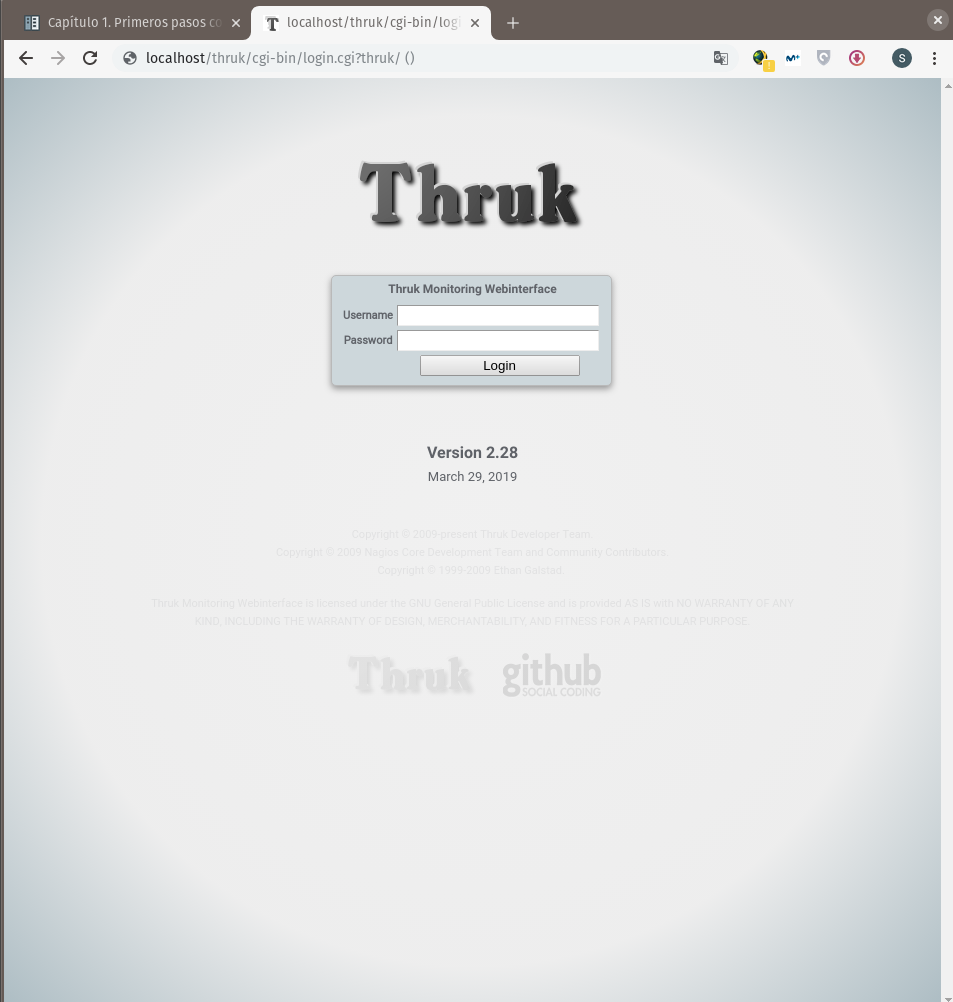
\includegraphics[width=0.7\textwidth]{imagenes/despliegue_naemon/ejecucionDocker.png}
	\caption{Ejecución de Docker} \label{run}
\end{figure}

\section{Orquestación de aplicaciones}

Existen múltiples definiciones sobre el concepto de \textbf{orquestación de aplicaciones} pero de un modo simple, podemos definir la \textbf{orquestación de servicios o aplicaciones} como el uso de la automatización para la creación y composición de la arquitectura, herramientas y procesos utilizados por operadores humanos para entregar un servicio.

La \textbf{orquestación} aprovecha tareas automatizadas y procesos predefinidos para permitir la creación de infraestructura complejas y para conseguir el aprovechamiento de los recursos de forma óptima y automatizada. Podemos considerar, a modo de analogía, el concepto de orquestación como un
proceso y la automatización como una tarea.
\newpage
De este modo, el objetivo principal de la orquestación consiste en la automatización de procesos orientados al despliegue y ciclo de vida de las aplicaciones o servicios. Y la automatización de procesos en los despliegues software se basan en el uso de algún tipo de software que facilite la instalación, configuración y mantenimiento del servicio o aplicación con la mínima intervención humana.

Existen dos tipos distintos de \textbf{orquestación} en base fundamentalmente a como se gestiona el escalado de recursos.
\begin{itemize}
	\item \textbf{Orquestación estática}: El sistema requiere una configuración más manual de los recursos y no permite el escalado de forma muy eficiente.
	\item \textbf{Orquestación Dinámica}: Escala de forma sencilla y eficientes los recursos de las aplicaciones y servicios y el propio sistema toma ciertas decisiones de forma automática.
\end{itemize}

En este proyecto, se plantea una solución de \textbf{orquestación estática} a través de la herramienta que cuenta Docker, llamada \textbf{Docker Compose} que permite la orquestación estática orientada a un funcionamiento más centrado un solo servidor, esta nos permite a través de un \textbf{fichero YML}, la definición y ejecución de aplicaciones Docker en múltiples contenedores.

Antes de comenzar con la explicación de \textbf{Docker Compose} explicaremos que es el formato \textbf{YML} o más bien conocido como \textbf{YAML} (Yet Another Markup Language). \cite{YML}

\textbf{YAML} se trata de un formato de serialización de datos de forma que sea legible para el usuario. Se inspira en lenguajes como XML, C, Python, Perl. Normalmente lo encontraremos con la extensión \textbf{.yml} o incluso \textbf{.yaml}.
\begin{figure}[H]
	\centering
	
\includegraphics[width=0.2\textwidth]{imagenes/despliegue_naemon/yaml.png}
	\caption{Logo de YAML} \label{yml}
\end{figure}
\newpage
Existen unas \textbf{reglas} generales que deben cumplirse en un documento \textbf{YAML} las principales son las siguientes:
\begin{itemize}
	\item Los datos de un documento YAML deben ser legibles, imprimibles y utilizando caracteres Unicode, UTF-8 ó UTF-16.
	\item Los comentarios se realizan utilizando el carácter \# dentro de la línea que contiene el comentario.
	\item Los caracteres , y ; deben ir seguidos de un espacio en blanco. De esta forma, se podrán representar valores que queramos que tengan esos caracteres.
	\item Los espacios en blanco están permitidos, pero no los tabuladores.
	\item Las listas comienzan por el caracter \textbf{``–"} con un valor por cada línea, aunque también se pueden utilizar corchetes \textbf{[]} poniendo los valores dentro de ellos separados por comas \textbf{``,"}junto con un espacio en blanco.
	\item Un vector estará formado por el par \textbf{clave/valor}, estando separados ambos por \textbf{``:"} poniendo uno por línea, aunque también podemos utilizar \textbf{{}} poniendo cada uno de ellos dentro separados por comas \textbf{``,"} junto con un espacio en blanco.
	\item Se pueden utilizar caracteres de escape \ para representar caracteres especiales.
\end{itemize}

\subsection{Uso de Docker Compose}

Como se ha mencionado se utilizará dicha herramienta para la ejecución de varios contenedores de Naemon trabajando de forma distribuida, pudiendo crear e iniciar todos a la vez.

Para ello tenemos que definir un fichero Dockerfile, ya lo tenemos creado.
Seguidamente crearemos un archivo llamado \textbf{docker-compose.yml} que se encargará de las ejecuciones del entorno.

Y para finalizar y reproducir la ejecución solo será necesario introducir a través de terminal desde la ruta en la que se encuentra el archivo de Docker Compose introducir:

\begin{lstlisting}[language=bash]
$ docker-compose up
\end{lstlisting}
\newpage
A continuación se comenta lo introducido en dicho archivo docker-compose.yml:

\begin{lstlisting}[language=bash]
version: '3.7'
services:
naemon:
build: .

ports:
- "32768:80"
image: "chui274/naemontfg"


\end{lstlisting}

Con la etiqueta version especificaremos la versión de Compose e incluyendo la versión de Docker Engine, por lo que si asignamos \textbf{version: '3.7'} estamos indicando que queremos la versión 3.7 de Docker Compose y la versión 18.06.0+ de Docker Engine.

A través de la etiqueta services comenzaremos a definir los contenedores que queremos crear, comenzamos creando nuestro contenedor llamado naemon, para la construcción es necesario la etiqueta build.

La etiqueta \textbf{build}  indicará la imagen de Dockerfile que vamos a usar, le indicamos . para que lea desde el archivo Dockerfile que se encontrará en el directorio principal.

Le indicaremos a través de la etiqueta \textbf{ports}   que realiza la escucha de la interfaz de thruk a través del puerto 32768.

Ahora a través de la etiqueta \textbf{image}  si hemos realizado la construcción bien con build, cogeremos la imagen desde chui274/naemontfg, que ha sido construida desde \textbf{.} .

Realizando el comando anterior mencionado a través de terminal, tendremos lo siguiente:

\begin{figure}[H]
	\centering
	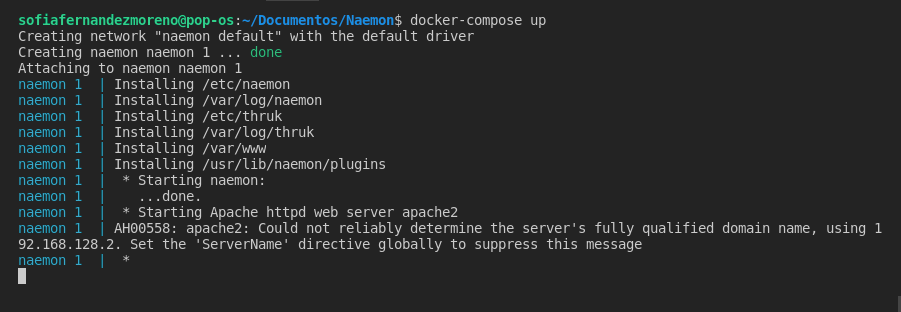
\includegraphics[width=1\textwidth]{imagenes/despliegue_naemon/terminal.png}
	\caption{Ejecución de Docker Compose} \label{dockercompose}
\end{figure}

Ahora estamos a disposición de probar la dirección \url{http://localhost:32768/} para acceder a Naemon a través de Thruk.

\begin{figure}[H]
	\centering
		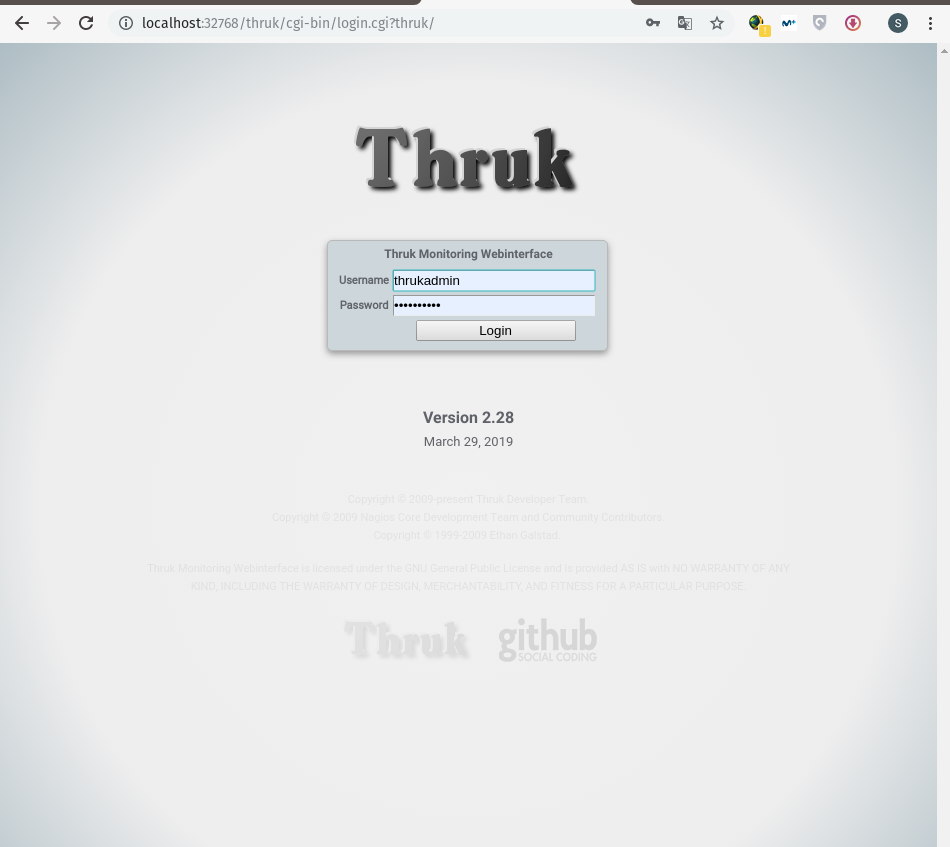
\includegraphics[width=1\textwidth]{imagenes/despliegue_naemon/pantallaDockerNaemon.png}
	\caption{Ejecución de Thruk mediante Docker Compose} \label{dockercomposethruk}
\end{figure}
\newpage